% kapitel2.tex
\chapter{Preliminaries}
\label{chapter:grundlagen}
Because the thesis covers many different systems each of them has to be introduces at least at a decent level. Modern and best of breed solution are being used here. Grafana and Prometheus are software products as a optional additional setup in cluster systems like kubernetes to monitor their technical values. As a little bonus and for easier developing process docker and docker compose will be used but in a very simple way. That technologies form the target of the \gls{dsl} designed in this thesis. For the realization of the \gls{dsl} and compiler Cinco, a meta modeling tool will be used.
 
\section{Smart Home}
In the course of digitalization and simplification of the procurement of sensor technology in everyday life, smart home has arrived as a concept for the consumer and is affordable. In the most general case, it is a base station with any number of actuators and sensors. This station is used to process and store the data from the sensory elements of the network and the actuators act on the basis of decision tables, for example. As a simple scenario, one can imagine a living room lamp that is switched on when the brightness sensor outside signals darkness. However, a system does not necessarily has to have sensors and actuators. A network of sensors would only monitor and one of actuators can only act. Examples would be a central power consumption monitoring per socket or a remote light control.
Here it is worth mentioning that there are also crossover devices. A heating thermostat usually has a built-in thermometer and is thus both actuator and sensor.\todo{add 1-2 par}\\

\begin{figure}[!h]
	\centering
	\begin{tikzpicture}[every text node part/.style={align=center}]
	\node[] (A) {
\includegraphics[width=50px]{./assets/images/plug-solid}\\sensor};
	\node[right= 3cm of A] (B) {
\includegraphics[width=50px]{./assets/images/chalkboard-solid}\\base station};
	\node[right= 3cm of B] (C) {
\includegraphics[width=50px]{./assets/images/lightbulb-solid}\\actuator};
	\draw[-{Stealth[scale=1.3,angle'=90]},semithick] (B) -- node[above] {0..N} (A) ;
	\draw[-{Stealth[scale=1.3,angle'=90]},semithick] (B) -- node[above] {0..M} (C) ;
	\end{tikzpicture}
	\caption{Abstract Smart Home Network}
\end{figure}
\todo{add source of images}
\section{Basic Terms}
In the context of Prometheus and this thesis, a few potentially ambiguous terms need to be specified more precisely.
\subsection{Metric}
A property which is observed and measured.
\begin{Beispiel}
	Temperature, rain amount, brightness, transfer rate, amount of printed documents
\end{Beispiel}
\begin{Definition}
	A metric is a single property to be measured.
\end{Definition}
\subsection{Sensor}
A sensor is a real device, a unit which is used in the real world. This can capture multiple metrics and then make them available via an interface.
\begin{Beispiel}
	Weather station, network switch, heating thermostat
\end{Beispiel}
\begin{Definition}
	A metric is a single property to be measured.
\end{Definition}

\section{Prometheus}
Prometheus is an open source solution that is used for metrics monitoring and alerting. There is the possibility to pass data actively or alternatively to configure Prometheus to fetch data from different data sources. For the latter variant, the system to be monitored must provide an \gls{http} interface on which the data is delivered in a predefined manner. Finally the collected data is persisted on the internal time series database.

To simplify this process, there are already several libraries for different programming languages that are configurable to export such a format. At the time of writing GO, Scala/Java, Python and Ruby are officially supported, but for many other languages there are unofficial third party libraries which are advertised on the Prometheus website. 

In case the selected language is not supported, it is also possible to create the output yourself. For this, the definition of the output format has been well documented.
\subsection{Metric Types}
Prometheus distinguishes between different types of metrics. In the following, all possibilities are briefly explained. In the \autoref{subsec:Exportformat} for understanding a few examples listed and explained.
\subsubsection{Counter}
The counter describes a metric type which can only be incremented and reset. It represents a monotonically growing function. 
\subsubsection{Gauge}
This type symbolizes a speedometer. The values can rise and fall.
\subsubsection{Histogram}
A histogram is a concept consisting of so-called buckets. These are initially defined for a metric. With the help of this definition, values of $]-\infty,+\infty[$ are sorted into the said buckets. Each next higher bucket also contains the measured values of the lower bucket. So it is a subset relation where the subsets are determined by the set limit. The \promcode{le} in the index can be interpreted as \textquote{Less Equal}. This parameter is also noted like this in the export.
\begin{figure}[htp!]
	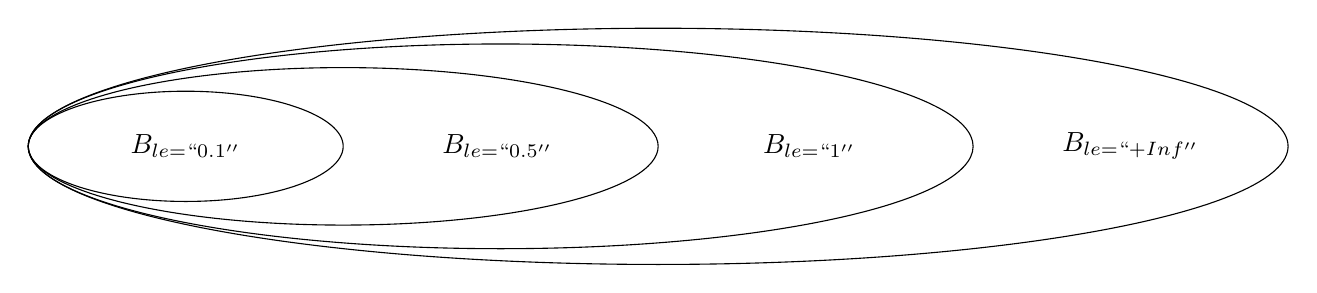
\begin{tikzpicture}
	\draw (0,0) ellipse (2cm and .7cm);
	\draw (2,0) ellipse (4cm and 1cm);
	\draw (4,0) ellipse (6cm and 1.3cm);
	\draw (6,0) ellipse (8cm and 1.5cm);
	\path (0,0) -- (12,0)%
	node[pos=0] {$B_{le=``0.1''}$}%
	node[pos=0.33] {$B_{le=``0.5''}$}%
	node[pos=0.66] {$B_{le=``1''}$}%
	node[pos=1] {$B_{le=``+Inf''}$};
	\end{tikzpicture}
	\caption{Relation of Bucket in a Histogram}
\end{figure}
A histogram represents, in addition to the buckets, a total number of measured values, which is like a bucket with \promcode{le="+Inf"} and a value for the sum of all values.
\begin{figure}[hbt!]
	\begin{minted}[mathescape,
	linenos,
	numbersep=5pt,
	gobble=0,
	frame=lines,
	linenos,
	tabsize=4,
	breaklines,
	framesep=2mm]{text}
	# TYPE <basename> histogram
	<basename>_bucket{le="<upper inclusive bound>"} <value>
	<basename>_sum <value>
	<basename>_count <value>
	\end{minted}
	\caption{General Concept of a Histogram Export}
\end{figure}
Line 2 can occur multiple times as each entry hat its own limit value. Lines 3 and 4 are the additional values as already mentioned.
\subsubsection{Summary}
\begin{figure}[h!]
	\begin{minted}[mathescape,
		linenos,
		numbersep=5pt,
		gobble=0,
		frame=lines,
		linenos,
		tabsize=4,
		breaklines,
		framesep=2mm]{text}
		# TYPE <basename> histogram
		<basename>{quantile="<φ>"} <value>
		<basename>_sum <value>
		<basename>_count <value>
	\end{minted}
	\caption{General Concept of a Summary Export}
\end{figure}
A summary is similar to a histogram, but here buckets are not filled by the value of the measurement but the measured values are divided into $\varphi$-quantiles ($0 \le \varphi \le 1)$ and the maximum value of the quantile.
\subsubsection{Untyped}
In this case a value is assigned to the metric without following any special rules. This is a safe default setting and it is inevitable not to use this type.
\Needspace{9\baselineskip}
\subsection{Labels}
Labels can be used to break down metrics with the same name into different origins. 
\begin{figure}[!ht]
	\begin{minted}[mathescape,linenos,numbersep=5pt,gobble=1,frame=lines,tabsize=4,breaklines,framesep=2mm]{text}
	<basename>{key="<value>",key2="<value2>",...} <value>
	\end{minted}
	\caption{General Concept of Labels}
\end{figure}
\subsection{Exportformat}
\label{subsec:Exportformat}
The export format of Prometheus can be described well by means of an example. For this purpose, we draw a part from the official documentation~\cite{PrometheusExpositionFormatBeispiel}.\\
\par
\begin{listing}[H]
	\begin{minted}[mathescape,linenos,numbersep=5pt,gobble=0,frame=lines,linenos,tabsize=4,breaklines,framesep=2mm]{text}
	# HELP http_requests_total The total number of HTTP requests.
	# TYPE http_requests_total counter
	http_requests_total{method="post",code="200"} 1027 1395066363000
	http_requests_total{method="post",code="400"}    3 1395066363000
	
	# Minimalistic line:
	metric_without_timestamp_and_labels 12.47
	\end{minted}
	\caption{Partial Example from the Official Prometheus Documentation~\cite{PrometheusExpositionFormatBeispiel}}
\end{listing}
Between lines 1-4 we find the first exported metric in this example. The first line contains after the token \promcode{# HELP <name of metric>} a short description which is Optional. The next line specifies the type with \linebreak \promcode{# TYPE <name of metric> <type of metric>}. The choices regarding the type coincide with the metric types already described: \promcode{counter}, \promcode{gauge}, \promcode{histogram}, \promcode{summary}, \promcode{untyped}.

All lines starting with \promcode{#} but not continued with \promcode{TYPE} or \promcode{HELP} are comment lines and therefore not interpreted.

Lines 3-4 show the measured values broken down by their labels. Lines that symbolize the measured values consist of three columns. The first in the format \promcode{<name of metric>} followed by optional labels in curly brackets. The example here breaks down all \gls{http} requests by method and \gls{http} return value. The next column contains the measured value for the metric, taking into account the optional grouping available. The last column is again non-mandatory and contains the timestamp at which the value was measured. 
In addition, we have a minimal example in line 7. Due to the lack of type specification, the type is \promcode{untyped}. The \gls{ebnf} to this type of line is as follows:
\begin{listing}[H]
	\begin{samepage}
		\begin{minted}[mathescape,
		linenos,
		numbersep=5pt,
		gobble=1,
		frame=lines,
		linenos,
		tabsize=4,
		breaklines,
		framesep=2mm]{ebnf}
		metric = metric_name, [ 
		"{",
		label_name, "=", '"', label_value, '"',
		{ ",", label_name, "=", '"', label_value, '"' }, [ "," ], 
		"}",
		],  value,  [ timestamp ];
		\end{minted}
		\caption{\gls{ebnf} following ISO/IEC 14977 of a Metric}
	\end{samepage}
\end{listing}

In the following lines you can see a more complex example. This is a histogram. The values measured internally in the exporter are divided into so-called buckets. You can see the four preconfigured buckets with the limits \promcode{0.05}, \promcode{0.2}, \promcode{1} and \promcode{+Inf}. 
\begin{listing}[H]
	\begin{minted}[mathescape,linenos,numbersep=5pt,gobble=1,frame=lines,tabsize=4,breaklines,framesep=2mm]{text}
	# HELP http_request_duration_seconds A histogram of the request duration
	# TYPE http_request_duration_seconds histogram
	http_request_duration_seconds_bucket{le="0.05"} 24054
	http_request_duration_seconds_bucket{le="0.2"} 100392
	http_request_duration_seconds_bucket{le="1"} 133988
	http_request_duration_seconds_bucket{le="+Inf"} 144320
	http_request_duration_seconds_sum 53423
	http_request_duration_seconds_count 144320
	\end{minted}
	\caption{Histogram Export Example from the Official Prometheus Documentation~\cite{PrometheusExpositionFormatBeispiel}}
\end{listing}
\todo{mention summary?}

\subsection{Prometheus Query Language}
As mentioned before, the collected data is stored in an internal Time Series database \todo{never mentioned} which can be searched by the so-called \gls{promql}.

There are four different subtypes for this:
\subsubsection{Instant vector}
Instant vector selectors allow the selection of a set of time series and a single sample value for each at a given timestamp (instant). In the simplest form, only a metric name is specified. This results in an instant vector containing elements for all time series that have this metric name. \todo{semantik der typen beschreiben}

\section{Grafana}
\label{sec:grafana}
For the visualization of the data collected by Prometheus, Grafana~\citep{GrafanaHomepage} can be used. It is a versatile and extensible system to display data from various data sources like databases like Cassandra, MariaDB or PostgreSQL but also regular \gls{http} requests against external interfaces or static \gls{json} objects are possible~\cite{GrafanaDataSources}. Furthermore, Grafana also provides different types of diagrams.
\todo{better layout, following fig.}
\begin{figure}[ht]
	\begin{subfigure}{.25\textwidth}
		\centering
		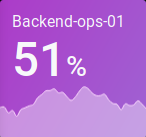
\includegraphics[width=.8\linewidth]{assets/screenshots/Screenshot_2020-12-08 1 - New Features in v7 0 - Grafana.png}
		\captionsetup{justification=centering}
		\caption{Single Metric\\with Graph}
		\label{fig:sfig1}
	\end{subfigure}%
	\begin{subfigure}{.25\textwidth}
		\centering
		
\includegraphics[width=.8\linewidth]{assets/screenshots/Screenshot_2020-12-08 Website trends - Grafana.png}
		\captionsetup{justification=centering}
		\caption{Single Metric\\as Gauge}
		\label{fig:sfig2}
	\end{subfigure}%
	\begin{subfigure}{.5\textwidth}
		\centering
		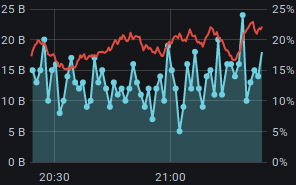
\includegraphics[width=.8\linewidth]{assets/screenshots/Screenshot_2020-12-08 Grafana Play Home - Grafana(2).png}
		\captionsetup{justification=centering}
		\caption{Multimetric plot}
		\label{fig:sfig2}
	\end{subfigure}
	\caption{Example Diagram Types in Grafana}
	\label{fig:fig}
\end{figure}
Supplementary there is a simple table format, honeycomb patterns, bar charts and many more. These, like the data sources, are extensible through plugins. Thanks to the source code openness of the project, custom plugins can be written if needed.

To fill the diagrams with data from, in our case, Prometheus, a \gls{promql} query must be stored in each diagram, which is executed regularly. Such a diagram is part of a so-called panel. That means, a panel has exactly one diagram and vice-versa. These are now combined into dashboards, which then provide an overview. Here you can define a lot of panels to display them at the same time.

It should also be said that there are higher order structures such as organizations or you can summarize dashboards again in playlists and / or groups. These features are not considered in this work however more near.

\subsection{Panels}
Since panels have many settings and thus allow many individualization, these are briefly explained here.

Each panel has primarily a name, description, diagram type, settings for the layout and value reference of cumulative functions and behavior with zero values. Depending on the selected chart type, different configurations are possible. Axis labeling, legend, limits for symbolic coloring and other specific settings.

Alternatively to the grouping of metrics, which is possible by keywords, it is a option to display several metrics in one diagram by specifying multiple \gls{promql} queries.

\section{Model Driven Development}


\section{Cinco}
Everything above is a necessary base technology where on top of it the model-driven solution, the domain specific language is build. For this task the meta modeling tool Cinco~\cite{CincoHomepage} will be used. The full name is \say{CINCO SCCE Meta Tooling Framework} and it utilizes the \gls{emf} and Graphiti Graphical Tooling Infrastructure. It is in active development of the chair for programming systems of the \gls{tudortmund}.

The \gls{mgl} allows the user to design a custom \gls{dsl} and generate a working \gls{ide} with features like auto complete, visual editing or code generation.

\todo{fig. from paper}

\todo{tell style language}

\subsection{Meta Graph Language}
Cinco uses four different elements for modeling a \gls{dsl} inside of it. The \gls{mgl}, which is used for that modeling task, defines nodes, edges, container and type elements. Having the ability of being enhanced with fields or dependencies between them they give the developer the opportunity designing a very powerful language. Basically the \gls{mgl} is like a graph with nodes and edges expanded with optional containers where a subset of the nodes and edges elements can be stored. The type node adds the ability of defining other needed types. In general there is also the feature of extending already defined types, so little adaptions can be done a a bigger level of abstraction can be implemented.

\subsubsection{Node}

A node is an unit which can have incoming and outgoing edges. It also can have different attributes and a so-called prime reference. A prime reference is a pointer to any other node, edge or container. This allows for example to make connections between different models in different files. Because Cinco is based on the \gls{emf} it is also possible to reference any other object defined in external sources. To declare a node the first token to use is \promcode{node} preceded by optional annotations and a optional \promcode{abstract} keyword. Followed by the name of the node and a declaring body wrapped in curly brackets. The body can contain definitions of attributes the node has to have, declaration of which edge types are incoming and which outgoing with optional constraints like quantities, a style option for correct visualization and a already described prime reference. An attribute starts with the keyword \promcode{attr}, like before there are other prefixes like final and unique. A type and a name are appended, optional minimal and maximal values and a default value. For the edges \promcode{incomingEdges} or \promcode{outgoingEdges} can be used with the possibility restricting the allowed edges and adding a cardinality to this declaration. Styles can be applied to the node by using the \promcode{style} keyword with a style id.
Further the last token \promcode{prime} is used for adding a prime reference to the node. It needs the referencing type and a name to be set up correctly.

\subsubsection{Edge}
Simpler constructs are edges. They are introduced using \promcode{edge} and can only contain attributes and a style. Like in the node definition annotations, abstraction flag or inheritance can be used without making cuts.

\subsubsection{Container}
Container heavily rely on the possibilities of a node. It is capable of all features of a node but being extended by the keyword \promcode{containableElements}. This makes it possible to allow specific object to be embedded inside of this container.

\subsubsection{Type}
Attributes can have different types. Cinco has therefor the following build-in datatypes:

\begin{center}
	EString | EChar | EFloat | EBoolean | EDouble | EInt | ELong | EBigInteger | EBigDecimal | EByte | EShort | EDate
\end{center}


The custom datatypes can either be enumerations or user defined types which are groups of attributes. Optional inheritance is also possible. Enums are defined by \promcode{enum} followed by a name and all possible literals. The user defined type uses the keyword \promcode{type}, a name and the list of attributes written down the same way like in the node definition.
